
%(BEGIN_QUESTION)
% Copyright 2006, Tony R. Kuphaldt, released under the Creative Commons Attribution License (v 1.0)
% This means you may do almost anything with this work of mine, so long as you give me proper credit

Calculate the voltage drops in this loop-powered 4-20 mA transmitter circuit for the current conditions shown in the table:

$$\includegraphics[width=15.5cm]{i00129x01.eps}$$

% No blank lines allowed between lines of an \halign structure!
% I use comments (%) instead, so that TeX doesn't choke.

$$\vbox{\offinterlineskip
\halign{\strut
\vrule \quad\hfil # \ \hfil & 
\vrule \quad\hfil # \ \hfil & 
\vrule \quad\hfil # \ \hfil & 
\vrule \quad\hfil # \ \hfil & 
\vrule \quad\hfil # \ \hfil & 
\vrule \quad\hfil # \ \hfil \vrule \cr
\noalign{\hrule}
%
% First row
Percent of range & Transmitter current & $V_{CD}$ & $V_{EF}$ & $V_{FG}$ & $V_{AB}$ \cr
%
\noalign{\hrule}
%
% Another row
0 \% & 4 mA &  &  &  &  \cr
%
\noalign{\hrule}
%
% Another row
25 \% & 8 mA &  &  &  &  \cr
%
\noalign{\hrule}
%
% Another row
50 \% & 12 mA &  &  &  &  \cr
%
\noalign{\hrule}
%
% Another row
75 \% & 16 mA &  &  &  &  \cr
%
\noalign{\hrule}
%
% Another row
100 \% & 20 mA &  &  &  &  \cr
%
\noalign{\hrule}
} % End of \halign 
}$$ % End of \vbox

In order for a loop-powered transmitter such as this to function adequately, there must be a minimum DC voltage between its terminals ($V_{AB}$) at all times.  A typical value for this voltage is 12 volts (be aware that this minimum voltage level varies considerably between different manufacturers and models!).  Identify what loop condition(s) may jeopardize this minimum supply voltage value, and how you as a technician would ensure the transmitter always received enough voltage to function.

\vskip 20pt \vbox{\hrule \hbox{\strut \vrule{} {\bf Suggestions for Socratic discussion} \vrule} \hrule}

\begin{itemize}
\item{} If a technician happened to be measuring transmitter terminal voltage while the pressure applied to the ``H'' port of the transmitter suddenly increased, would the measured voltage increase or decrease?  
\item{} This circuit shows {\it two} resistors, rather than just one.  Identify a practical reason why a 4-20 mA loop circuit might have multiple resistances in it.
\item{} Demonstrate how to {\it estimate} numerical answers for this problem without using a calculator.
\end{itemize}

\underbar{file i00129}
%(END_QUESTION)





%(BEGIN_ANSWER)

% No blank lines allowed between lines of an \halign structure!
% I use comments (%) instead, so that TeX doesn't choke.

$$\vbox{\offinterlineskip
\halign{\strut
\vrule \quad\hfil # \ \hfil & 
\vrule \quad\hfil # \ \hfil & 
\vrule \quad\hfil # \ \hfil & 
\vrule \quad\hfil # \ \hfil & 
\vrule \quad\hfil # \ \hfil & 
\vrule \quad\hfil # \ \hfil \vrule \cr
\noalign{\hrule}
%
% First row
Percent of range & Transmitter current & $V_{CD}$ & $V_{EF}$ & $V_{FG}$ & $V_{AB}$ \cr
%
\noalign{\hrule}
%
% Another row
0 \% & 4 mA & 24 V & 1 V & 0.2 V & 22.8 V \cr
%
\noalign{\hrule}
%
% Another row
25 \% & 8 mA & 24 V & 2 V & 0.4 V & 21.6 V \cr
%
\noalign{\hrule}
%
% Another row
50 \% & 12 mA & 24 V & 3 V & 0.6 V & 20.4 V \cr
%
\noalign{\hrule}
%
% Another row
75 \% & 16 mA & 24 V & 4 V & 0.8 V & 19.2 V \cr
%
\noalign{\hrule}
%
% Another row
100 \% & 20 mA & 24 V & 5 V & 1 V & 18 V \cr
%
\noalign{\hrule}
} % End of \halign 
}$$ % End of \vbox

The Rosemount 3144 temperature transmitter, for example, requires a minimum of 12 volts at its terminals to function in the analog mode, and 18.1 volts in order to properly function while communicating using the HART digital-over-analog protocol.  Note how the operation of such a 3144 transmitter in a loop with a 24 volt power supply and 300 ohms worth of resistance would be jeopardized near the upper end of the signal range.

%(END_ANSWER)





%(BEGIN_NOTES)


%INDEX% Basics, loop-powered transmitter: voltage drop calculations

%(END_NOTES)


